\documentclass[11pt,a4paper]{article}

\usepackage{verbatim}
\usepackage{fancyhdr}           % For header and footer
\usepackage{multicol}           % Allows multicols in tables
\usepackage{graphicx}           % For images
\usepackage{xcolor}             % For hex colours
\usepackage{colortbl}           % For coloured tables
\usepackage{setspace}           % For line height
\usepackage{seqsplit}           % Splits long words.
\usepackage{amsmath}            % Symbols

\graphicspath{{../Images/}}
% Lengths and widths
\addtolength{\textwidth}{5cm}
\addtolength{\hoffset}{-1cm}
\setlength{\headsep}{-12pt} % Reduce space between header and content
\setlength{\headheight}{85pt} % If less, LaTeX automatically increases it
\renewcommand{\footrulewidth}{2pt} % Remove footer line
\renewcommand{\headrulewidth}{1pt} % Remove header line
\renewcommand{\seqinsert}{\ifmmode\allowbreak\else\-\fi} % Hyphens in seqsplit
% This two commands together give roughly
% the right line height in the tables
\renewcommand{\arraystretch}{1.3}
\onehalfspacing



% Commands
\newcommand{\SetRowColor}[1]{\noalign{\gdef\RowColorName{#1}}\rowcolor{\RowColorName}} % Shortcut for row colour
\newcommand{\mymulticolumn}[3]{\multicolumn{#1}{>{\columncolor{white}}#2}{#3}} % For coloured multi-cols
\newcolumntype{x}[1]{>{\raggedright}p{#1}} % New column types for ragged-right paragraph columns
\newcommand{\tn}{\tabularnewline} % Required as custom column type in use

% Font and Colours
\definecolor{HeadBackground}{HTML}{333333}
\definecolor{FootBackground}{HTML}{666666}
\definecolor{TextColor}{HTML}{333333}
\definecolor{DarkBackground}{HTML}{6B8E23} %{FD1AA8}
\definecolor{LightBackground}{HTML}{E8FED8} %D3FDC8
\definecolor{tit}{HTML}{FF6600}
\renewcommand{\familydefault}{\sfdefault}
\color{TextColor}
 \headsep = 25pt
% Header and Footer
\pagestyle{fancy}
\usepackage[headheight=110pt]{geometry}
\fancyhf{}% Clear header/footer

\fancyhead[r]{
\includegraphics[width = 4cm, height = 2cm]{TS-Logo.png}\hspace{0cm}}
\fancyhead[l]{\Large{\bf{\textcolor{tit}{\textrm{Joins and Subqueries}}}}}

\renewcommand{\headrulewidth}{0.4pt}% Default \headrulewidth is 0.4pt
\renewcommand{\footrulewidth}{0.4pt}% Default \footrulewidth is 0pt

\rfoot{Page \thepage}
\lfoot{COPYRIGHT \textcopyright TALENTSPRINT, 2015. ALL RIGHTS RESERVED.}

\begin{document}
\vspace{5in}

Joins are used to query data from two or more tables, based on a relationship between certain columns in these tables. There are different types of JOINing methods used in MySQL database, which are given below.

\subsubsection*{INNER JOIN} Probably the most common join operation MySQL supports is an inner join. It identifies and combines only matching rows which are stored in two or more related tables.

A join condition, which indicates how the tables are related, is added with the keywords ON or USING.

NOTE:

\textbf{ON is used when the relationship column names are different.}

\textbf{USING is used when the relationship column names are same.}
\subsubsection*{INNER JOIN with ON clause}
\textbf{Syntax}
\begin{verbatim}
SELECT <column list> FROM tableA a INNER JOIN tableB b ON a.somecolumn = b.othercolumn;
\end{verbatim}

\textbf{Example}
\begin{verbatim}
mysql> SELECT d.deptno, d.dname, e.empno, e.ename FROM dept d INNER JOIN emp e ON d.deptno = e.deptid;\end{verbatim}
\subsubsection*{INNER JOIN with USING clause syntax}
\textbf{Syntax}
\begin{verbatim}
SELECT * FROM tableA a INNER JOIN tableB b USING(columnname);\end{verbatim}

\textbf{Example}
\begin{verbatim}
SELECT d.deptno, d.dname, e.empno, e.ename FROM dept d INNER JOIN emp e USING (deptno);\end{verbatim}
\subsubsection*{OUTER JOIN} OUTER JOIN allows us to retrieve all values in a certain table regardless of whether these values are present in other tables.\\

The difference between inner and outer join is: An outer join can identify rows without a match in the joined table. When no match was found, MySQL sets the value of
columns from the joined table to NULL.\\

\subsubsection*{LEFT OUTER JOIN} This type of join will display matching records from both tables and all unmatched records of the left table. Left table means which table name is listed on the left side of the JOIN keywords.\\

\textbf{Syntax}
\begin{verbatim}
SELECT <column list> FROM table1 a LEFT OUTER JOIN table2 b ON a.somecolumn = b.othercolumn;\end{verbatim}

\textbf{Example}
\begin{verbatim}
SELECT d.deptno, d.dname, e.empno, e.ename FROM dept d LEFT OUTER JOIN employees e 
    ON d.deptno = e.deptnumber;\end{verbatim}

\subsubsection*{RIGHT OUTER JOIN} This type of join will display matching records from both tables and all unmatched
records of the right table. Right table means which table name is listed on the right side of the JOIN keywords.

\textbf{Syntax}
\begin{verbatim}SELECT <column list> FROM table1 a RIGHT OUTER JOIN table2 b ON a.somecolumn = b.othercolumn;\end{verbatim}

\textbf{Example}
\begin{verbatim}
SELECT d.deptno, d.dname, e.empno, e.ename FROM dept d RIGHT OUTER JOIN employees e 
    ON d.deptno = e.deptnumber;\end{verbatim}

\subsubsection*{SELF JOIN} A self-join, also known as an inner join, is a structured query language (SQL) statement where a queried table is joined to itself. The self-join statement is necessary when two sets of data, within the same table, are compared.

\textbf{Example} Suppose you're tasked with writing a SQL query to retrieve a list of employees and their managers.
\begin{verbatim}mysql> SELECT e.firstname AS `Employee FN', e.lastname AS `Employee LN', 
    m.firstname AS `Manager FN', m.lastname AS `Manager LN' 
    FROM employees AS e LEFT OUTER JOIN employees AS m ON e.manager =m.id;\end{verbatim}

\subsubsection*{CROSS JOIN} The cross join operation retrieves data between two tables as a Cartesian product of set theory in mathematics. Each row will get multiplied by other rows. If one table has three rows and the second row has two rows, then the Cartesian of two table will be six. 

\textbf{Example}

\begin{verbatim}mysql> SELECT * FROM dept CROSS JOIN employee;\end{verbatim}
\section*{SubQueries}
A subquery is a SQL query nested inside a larger query.\\

A subquery may occur in :\\
\textbf{A SELECT clause}\\
\textbf{A FROM clause}\\
\textbf{A WHERE clause}\\

In MySQL subquery can be nested inside a SELECT, INSERT, UPDATE, DELETE, SET, or DO statement or inside another subquery.

A subquery is usually added within the WHERE Clause of another SQL SELECT statement.
You can use the comparison operators, such as $>$, $<$, or $=$. The comparison operator can also be a multiple-row operator, such as IN, ANY, SOME, or ALL.
A subquery can be treated as an inner query, which is a SQL query placed as a part of another query called as outer query.
The inner query executes first before its parent query so that the results of inner query can be passed to the outer query.

\textbf{Syntax}
\begin{verbatim}

SELECT select_list from outerTable where expr_operator(SELECT select_list from innerTable);\end{verbatim}
In the above statement the inner query will be parsed first and the result will be passed to the outer query.
\subsubsection*{Types of SubQueries}
\begin{itemize}
 \item Scalar SubQueries
 \item SubQueries with ANY,ALL,IN
 \item SubQueries with EXISTS and NOT EXISTS
 \item Correlated SubQueries
 \end{itemize}
\subsubsection*{Scalar SubQueries}
\begin{itemize}
 \item A scalar subquery is a subquery that returns exactly one column value from one row.
 \item If the subquery returns 0 rows then the value of scalar subquery expression in NULL.
 \item If the subquery returns more than one row then MySQL returns an error.
 \item The subquery can be used in either SELECT statement or WHERE clause.
 \item In either case, an aggregate function or an expression is normally used in the subquery.
 \item When the subquery is used in WHERE clause, a comparison operator is always used
\end{itemize}
\subsubsection*{Subquery in WHERE clause with an aggregate function}
\begin{verbatim}
 mysql>select OrderID, CustomerID from orders where 
     ShippedDate = (select max(ShippedDate) from orders);\end{verbatim}
\begin{figure}[ht]
\begin{center}
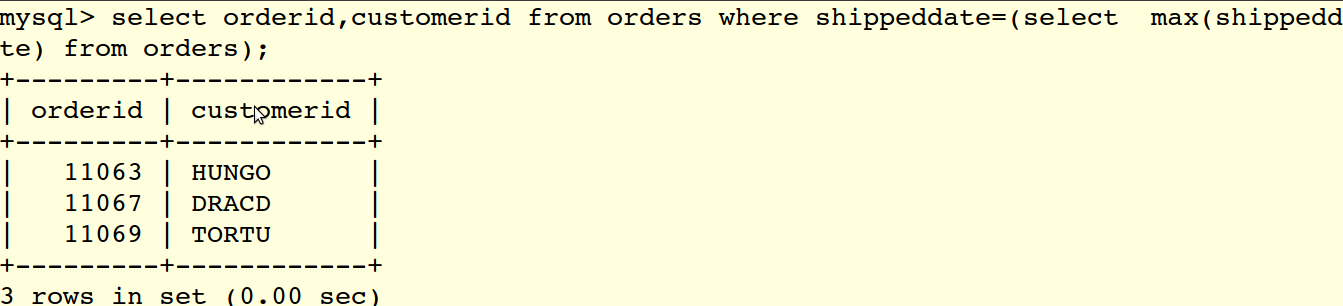
\includegraphics[scale=0.3]{max.png}
\caption{figure}{Scalar SubQuery using Max function}
\end{center}
\end{figure}  
NOTE:The above query returns data for all customers and their orders where the orders were shipped on the most recent recorded day.
\begin{verbatim}
mysql>select distinct ProductName, UnitPrice from products 
    where UnitPrice>(select avg(UnitPrice) from products) order by UnitPrice desc;\end{verbatim}

NOTE:This query returns all products whose unit price is greater than average unit price of all Products.

\subsubsection*{SubQueries using ALL}
The ALL keyword specifies that the search condition is TRUE if the comparison is TRUE for every value that the subquery returns.

In the following example, the first condition tests whether each unitprice is greater than the unitprice of productid=1.
\begin{verbatim}
mysql>select productname,unitprice from products where unitprice > ALL 
    (SELECT unitprice FROM products WHERE productid = 1);\end{verbatim}

\begin{figure}[ht]
\begin{center}
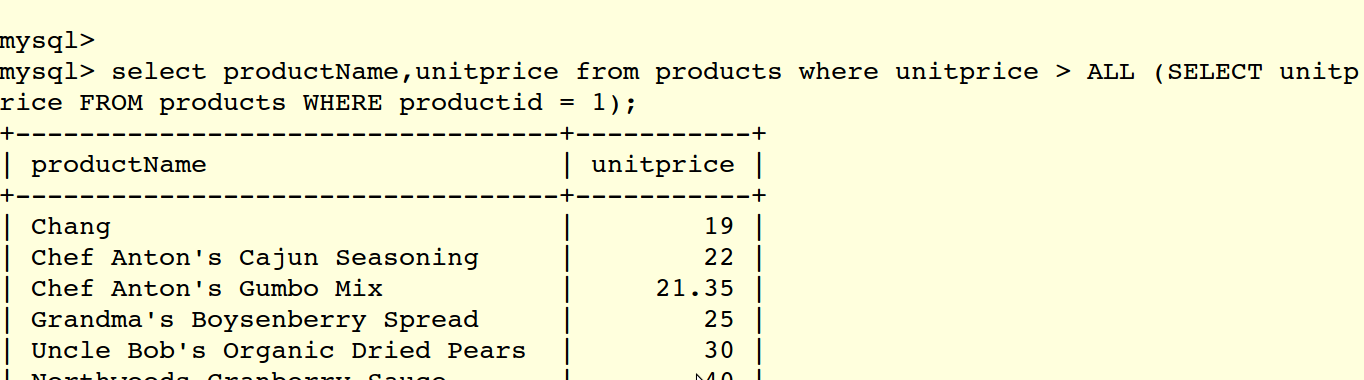
\includegraphics[scale=0.3]{all.png}
\caption{figure}{Subquery using ALL}
\end{center}
\end{figure}

\subsubsection*{Subquery using ANY}
The ANY keyword denotes that the search condition is TRUE if the comparison is TRUE for at least one of the values that is returned. If the subquery returns no value, the search condition is FALSE. The SOME keyword is a synonym for ANY.
\begin{verbatim}
mysql>select productName,unitprice from products 
    where unitprice < ANY (SELECT unitprice FROM products WHERE productid = 1);\end{verbatim}
\begin{figure}[ht]
\begin{center}
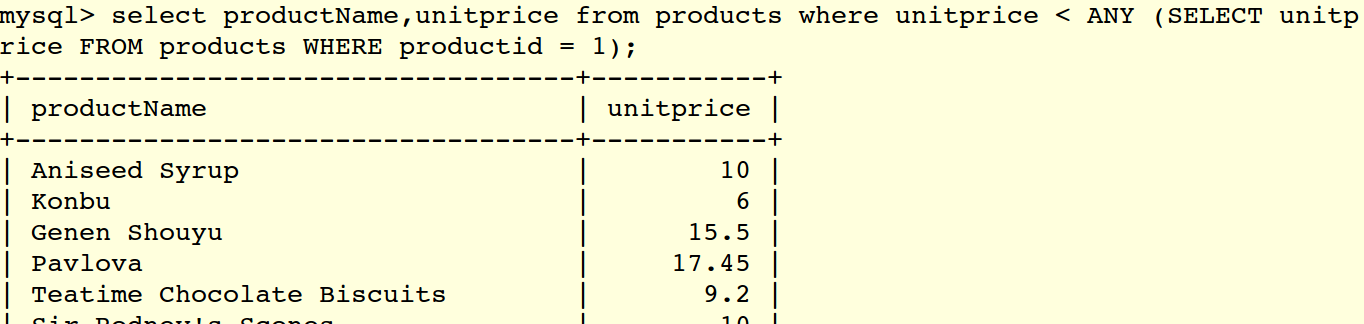
\includegraphics[scale=0.3]{any.png}
\caption{figure}{SubQuery using ANY}
\end{center}
\end{figure}  
\subsubsection*{Subquery using EXISTS}
The MySQL EXISTS condition is used in combination with a subquery and is considered ``to be met'' if the subquery returns at least one row. It can be used in a SELECT, INSERT, UPDATE, or DELETE statement.

\textbf{NOTE:SQL statements that use the EXISTS Condition in MySQL are very inefficient since the sub-query is RE-RUN for EVERY row in the outer query's table.}
\begin{verbatim}
mysql>select * from customers where EXISTS (select * from order_details
    where customers.customer_id = orders.customer_id);\end{verbatim}
\begin{figure}[h]
\begin{center}
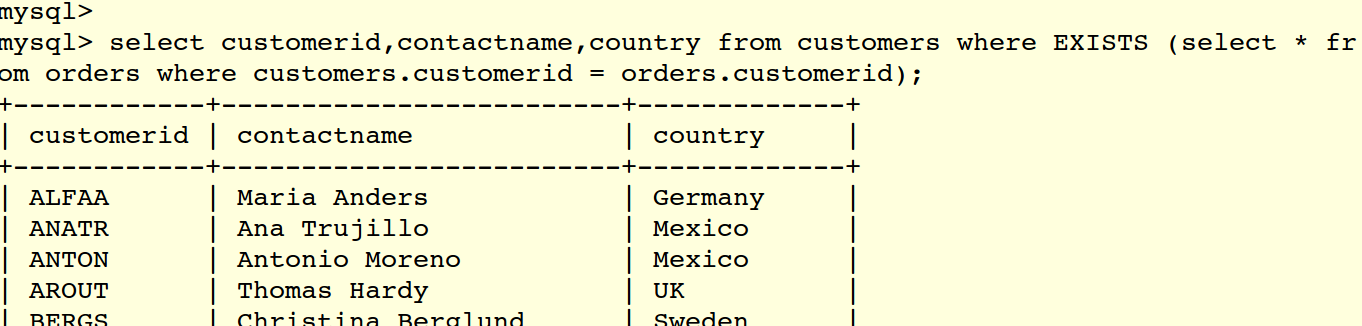
\includegraphics[scale=0.3]{exists.png}
\caption{figure}{Exists Condition}
\end{center}
\end{figure}  
NOTE:The above example will return all records from the customers table where there is at least one record in the order\_details table with the matching customer\_id.

\subsubsection*{Subquery using NOT EXISTS}
\begin{verbatim}
select * from customers where NOT EXISTS (select * from order_details 
    where customers.customer_id = orders.customer_id);\end{verbatim}
\begin{figure}[h]
\begin{center}
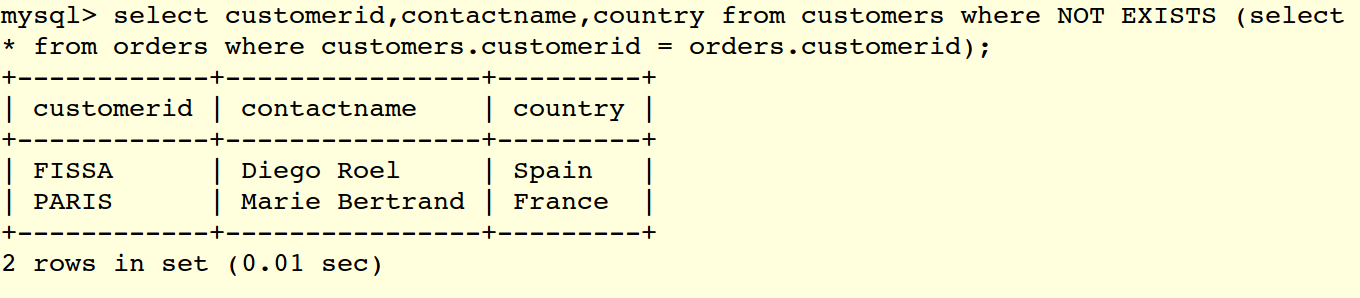
\includegraphics[scale=0.3]{notexists.png}
\caption{figure}{Not Exists Condition}
\end{center}
\end{figure}  
NOTE:The above example will return all records from the customers table when there are no records in the order\_details table for the given customer\_id.
\subsubsection*{Subquery using EXISTS and INSERT}
\begin{verbatim}INSERT into contacts (contact\_id, contact\_name) 
    select supplier\_id, supplier\_name from suppliers 
    where EXISTS (select * from orders 
    where suppliers.supplier\_id = orders.supplier\_id);\end{verbatim}
NOTE:The above example will insert records into contacts table if supplier\_id of suppliers and orders table matches.                                                                
\subsubsection*{Subquery using EXISTS and DELETE}
\begin{verbatim}DELETE from suppliers where EXISTS 
    (select * from orders where suppliers.supplier_id = orders.supplier_id);\end{verbatim}
NOTE:The above example will delete records from suppliers table if supplier\_id of suppliers and orders table matches.                                                        

\subsubsection*{Correlated SubQueries}
A correlated subquery is a subquery that contains a reference to a table (in the parent query) that also appears in the outer query.\\
MySQL evaluates from inside to outside.
\begin{verbatim}
mysql> select supplierid, productname from products p 
    where unitprice > (select AVG(unitprice) from products where supplierid = p.supplierid);\end{verbatim}
\begin{figure}[ht]
\begin{center}
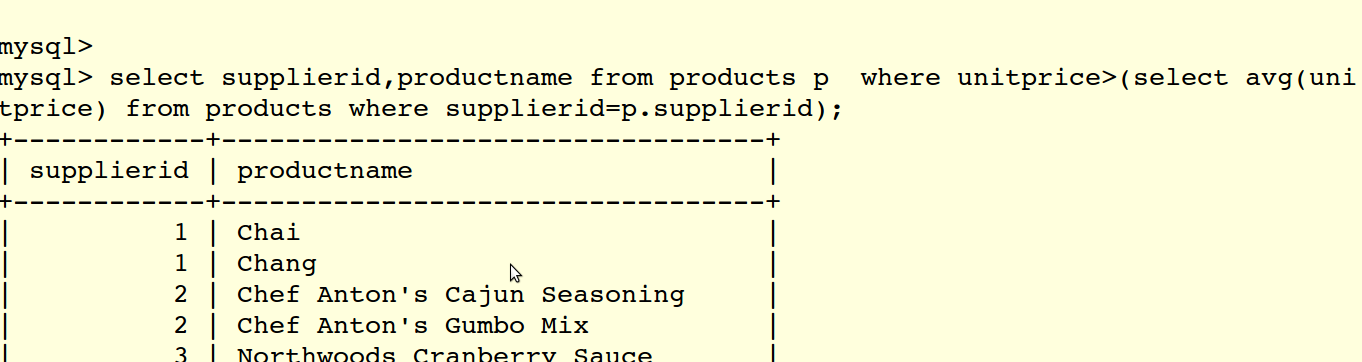
\includegraphics[scale=0.2]{corel.png}
\caption{figure}{Correlated SubQuery}
\end{center}
\end{figure}
Displaying all employees whose salary is greater than the average salary of their own department.

\end{document}
